\section{Résultats du calcul automatique}\label{sec:pred_stationnement}
Une estimation réglementaire de stationnement a été calculée pour l'ensemble des propriétés dans les limites de la ville de Québec. Les graphiques présentés dans cette section ont été générés avec des scripts Python dédiés pour améliorer la lecture. La source est disponible dans un dépôt Github \parencite{charbonneau_epmpaulpolygraphiques_memoire_2025}.  Dans cette section, les prédictions seront présentées en utilisant les minimums calculés sauf indication contraire. Au total, la méthode réglementaire donne une estimation de 498 800 places de stationnement. La figure \ref{fig:result-dist-places-par-usage} montre la distribution des places de stationnement entre les différents usages du sol.\par
\begin{figure}[!h]
    \centering
    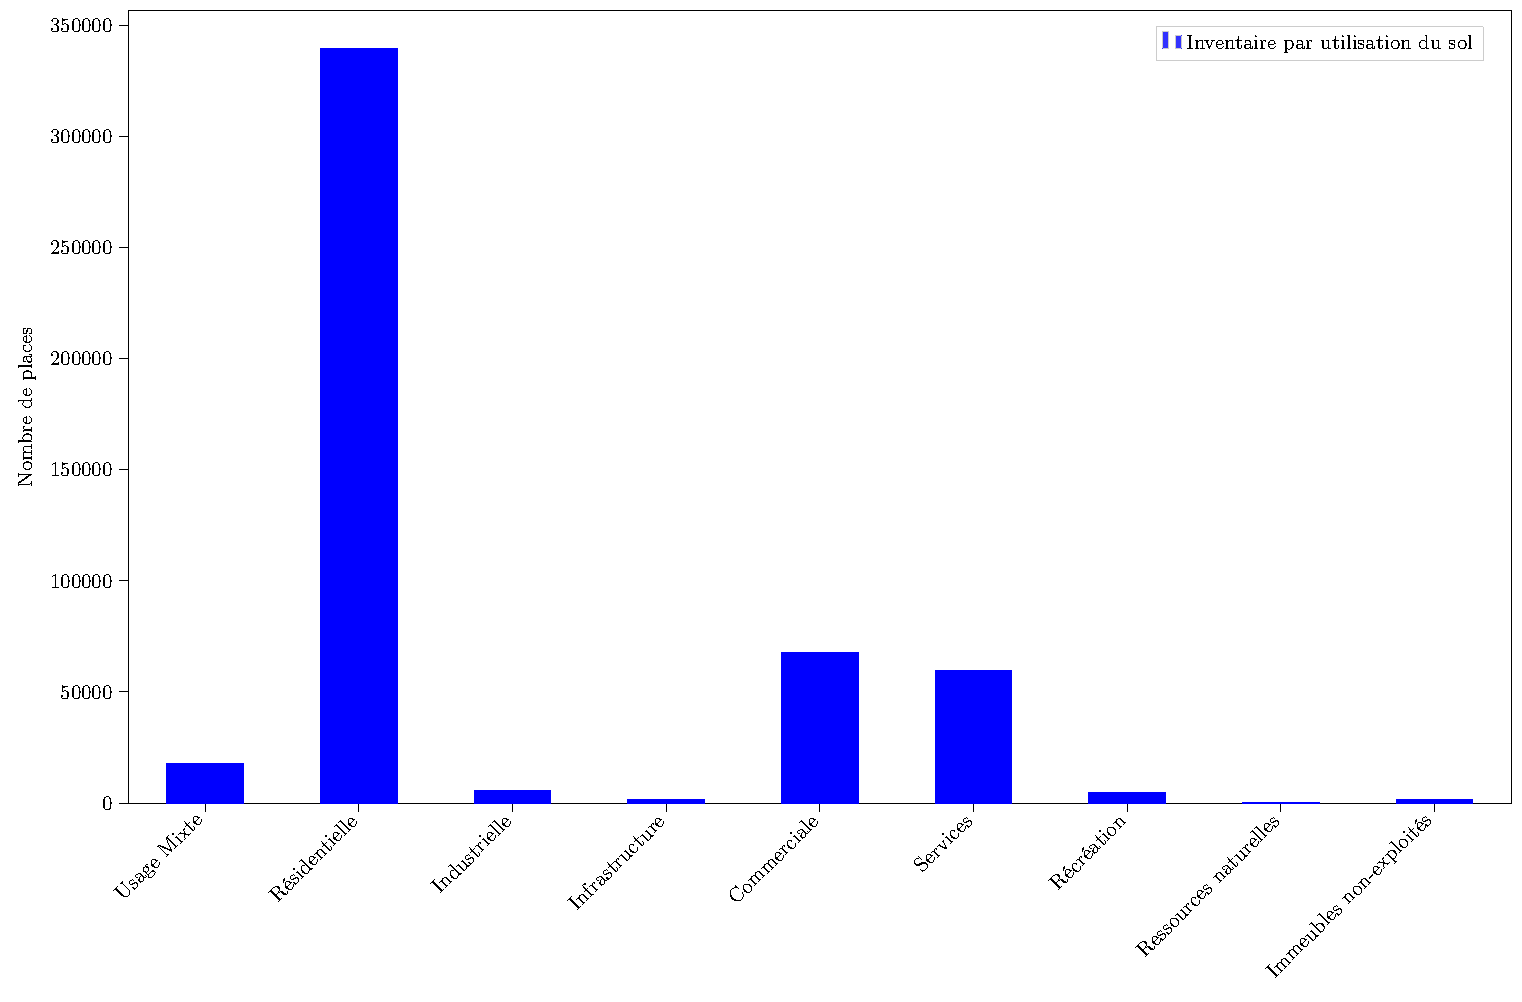
\includegraphics[width=0.75\textwidth]{figures/inventaire-reg-par-cubf.pdf}
    \caption{Distribution des places des stationnements par utilisation du sol}
    \label{fig:result-dist-places-par-usage}
\end{figure}
Le modèle prédit que les stationnements résidentiels (305 700 places) constituent 65\% du parc de stationnement hors rue. Les propriétés commerciales (67 000 places de stationnement) et de services (58 800 places de stationnement) sont les deux autres grands contributeurs à la capacité prédite. Ce constat est émis sous réserve puisqu'une partie importante de la valeur foncière à ces deux postes n'a pas les données requises (cf. sec. \ref{ssec:analyse-descriptive-role-fonc}) . \par 
\FloatBarrier
Ce parc de stationnement n'est pas uniformément réparti. Les figures \ref{fig:result-dist-places-par-quartier} et \ref{fig:n-places-reg-carto} montrent la distribution spatiale du parc de stationnement dans la ville de Québec selon les quartiers administratifs. Le modèle prédit que les secteurs Duberger-Les Saules et Neufchatel-Est et la Cité Universitaire contiennent une grande partie du parc de stationnement hors rue. Les acronymes utilisés sont ceux donnés au tableau \ref{tab:acro-quartiers}. 
\begin{figure}[H]
    \centering
    \begin{subfigure}[b]{0.9\textwidth}
        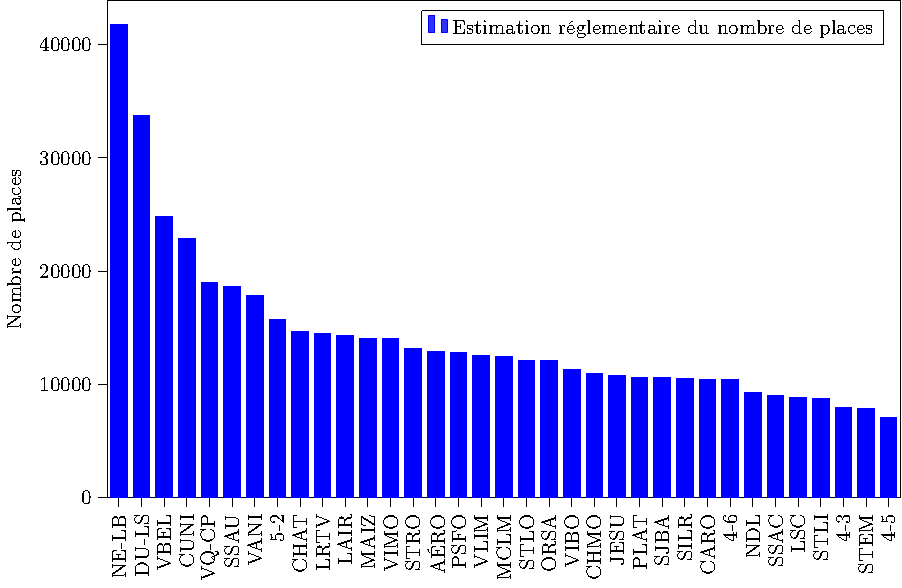
\includegraphics[width=0.9\linewidth]{figures/inventaire-reg-par-quartier.pdf}
        \caption{Histogramme}
        \label{fig:result-dist-places-par-quartier}
    \end{subfigure}
    ~
    \begin{subfigure}[b]{0.9\textwidth}
        \centering
        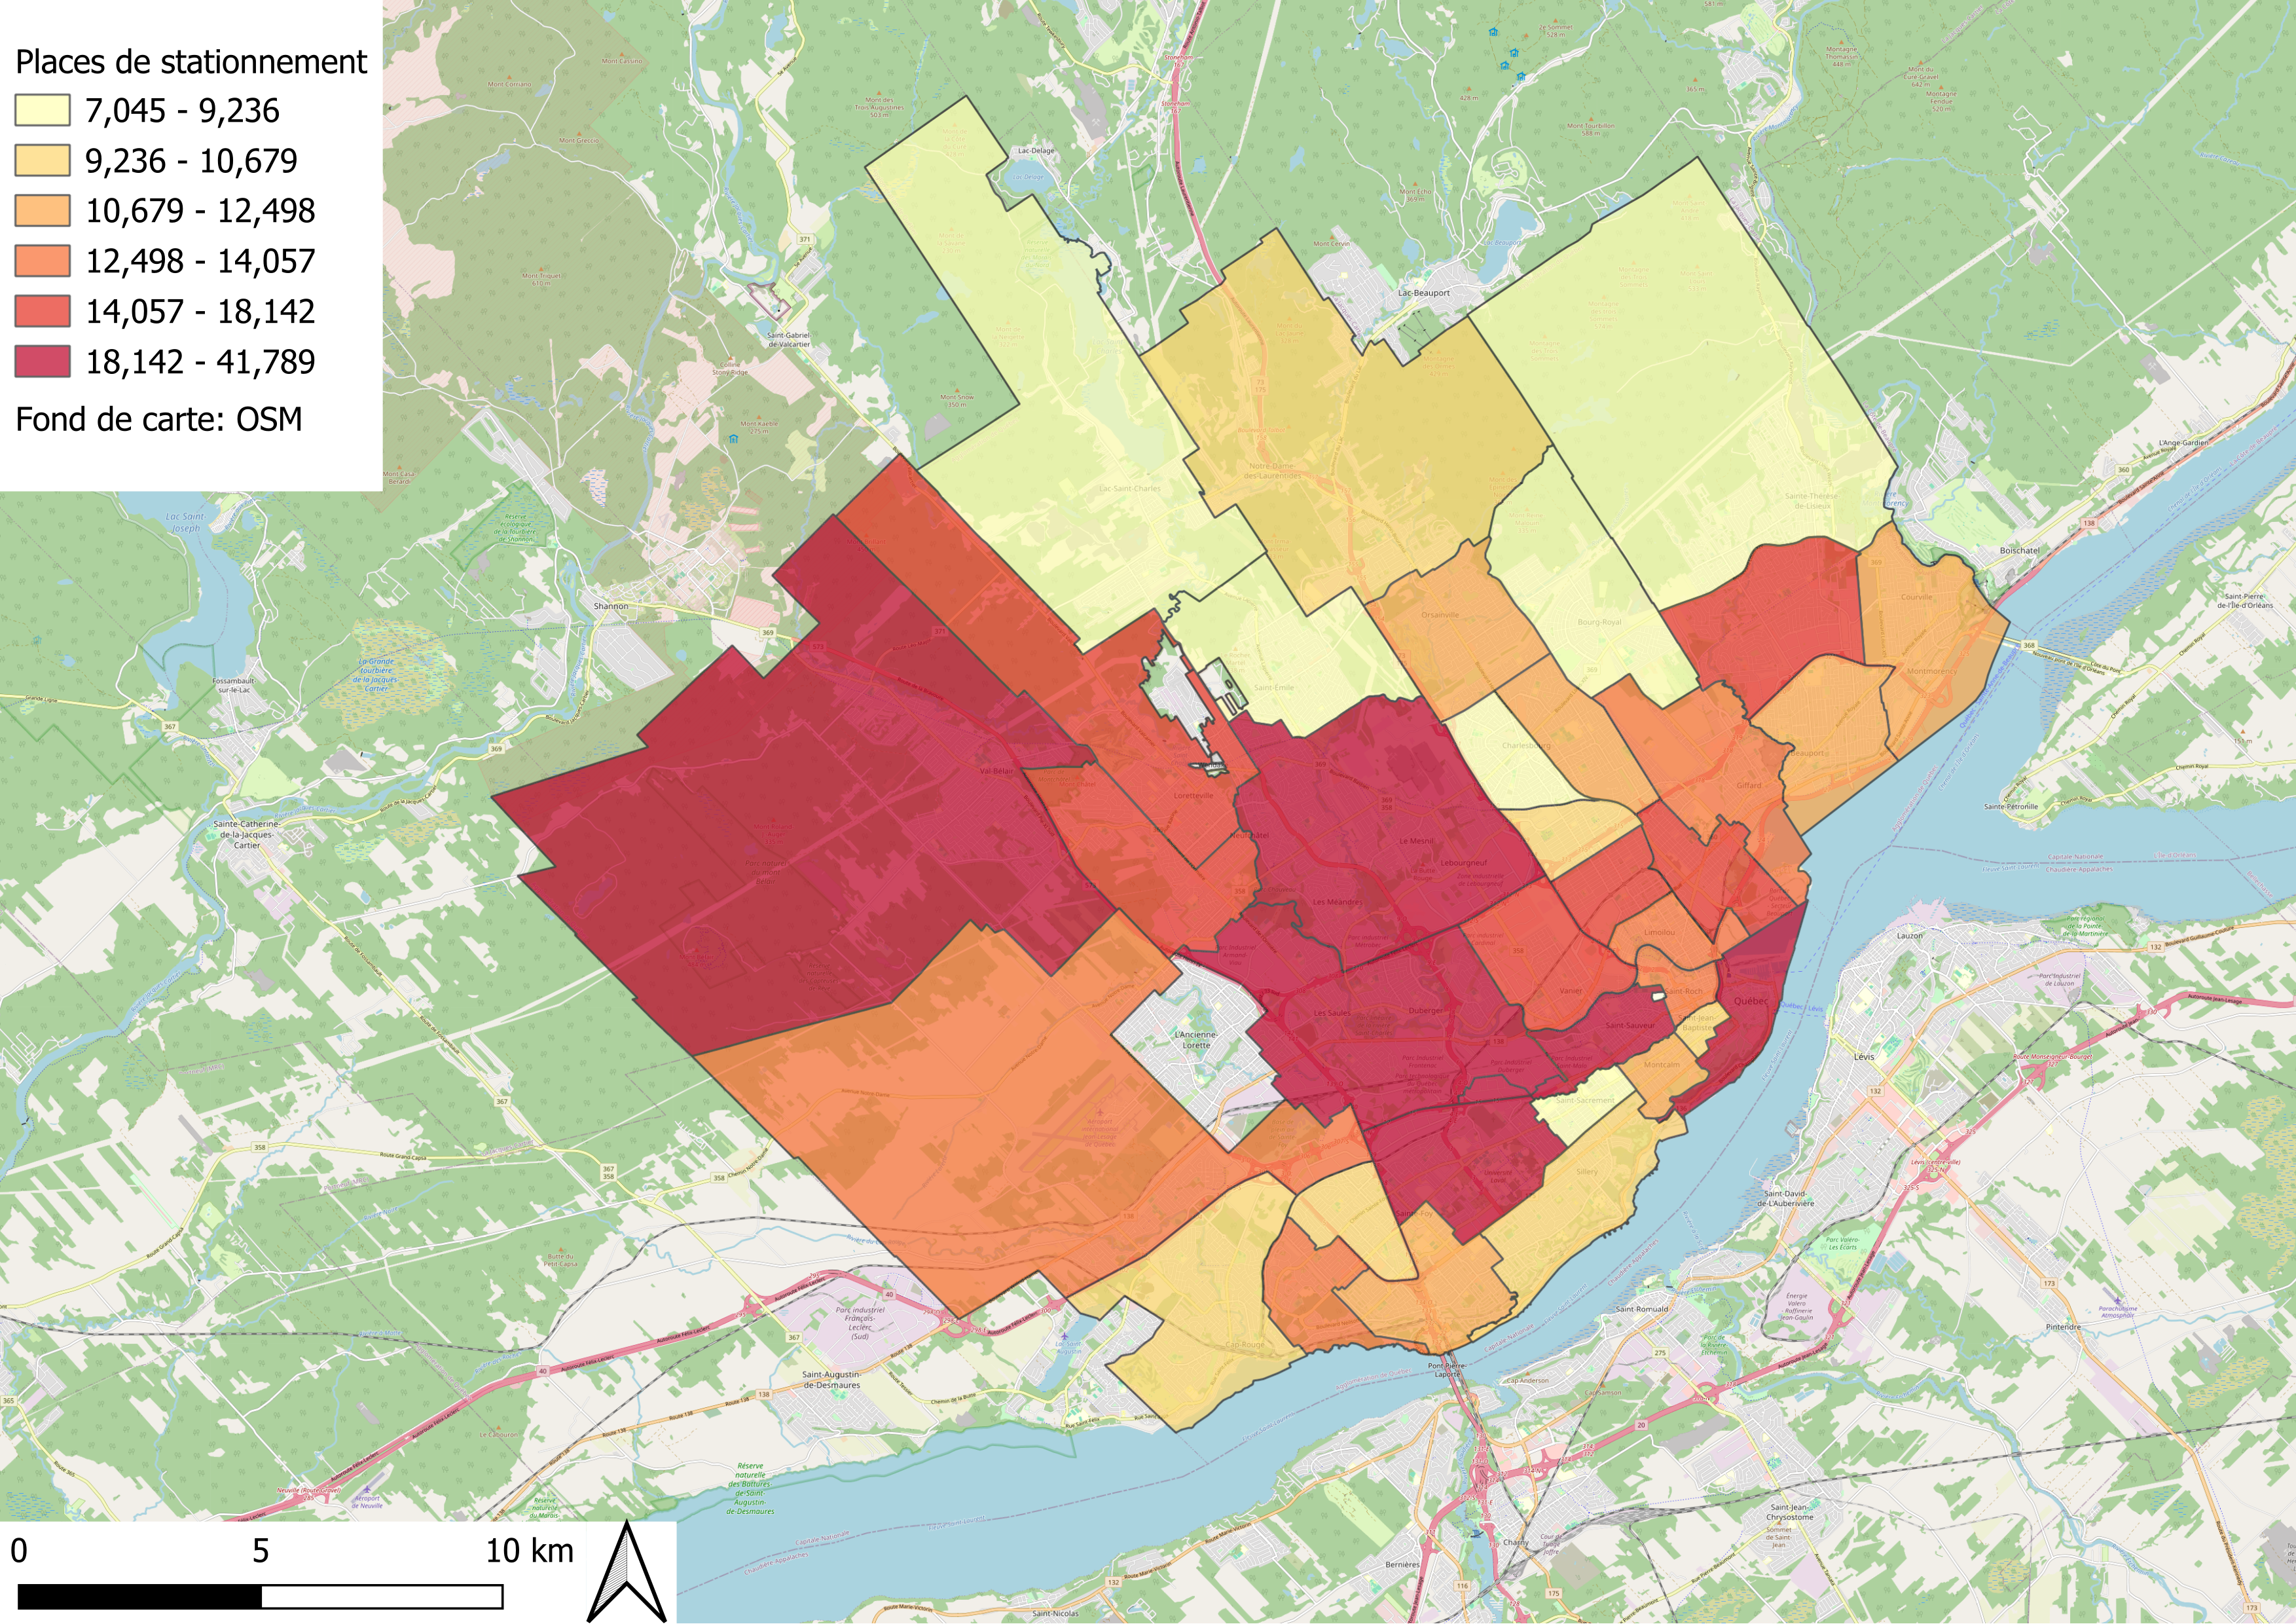
\includegraphics[width=0.9\linewidth]{images/n-places-reg.png}
        \caption{Carte}
        \label{fig:n-places-reg-carto}
    \end{subfigure}
    \caption{Distribution des places de stationnement sur le territoire}
\end{figure}
\FloatBarrier
La densité de stationnement suit essentiellement le même schéma que la densité de population comme le montrent les figures \ref{fig:dens-pop} et \ref{fig:dens-stat}.
L'exception est la colline Parlementaire qui a un excédent de stationnements par rapport à sa population. 
\begin{figure}[!h]
    \centering
    \begin{subfigure}[b]{0.725\textwidth}
        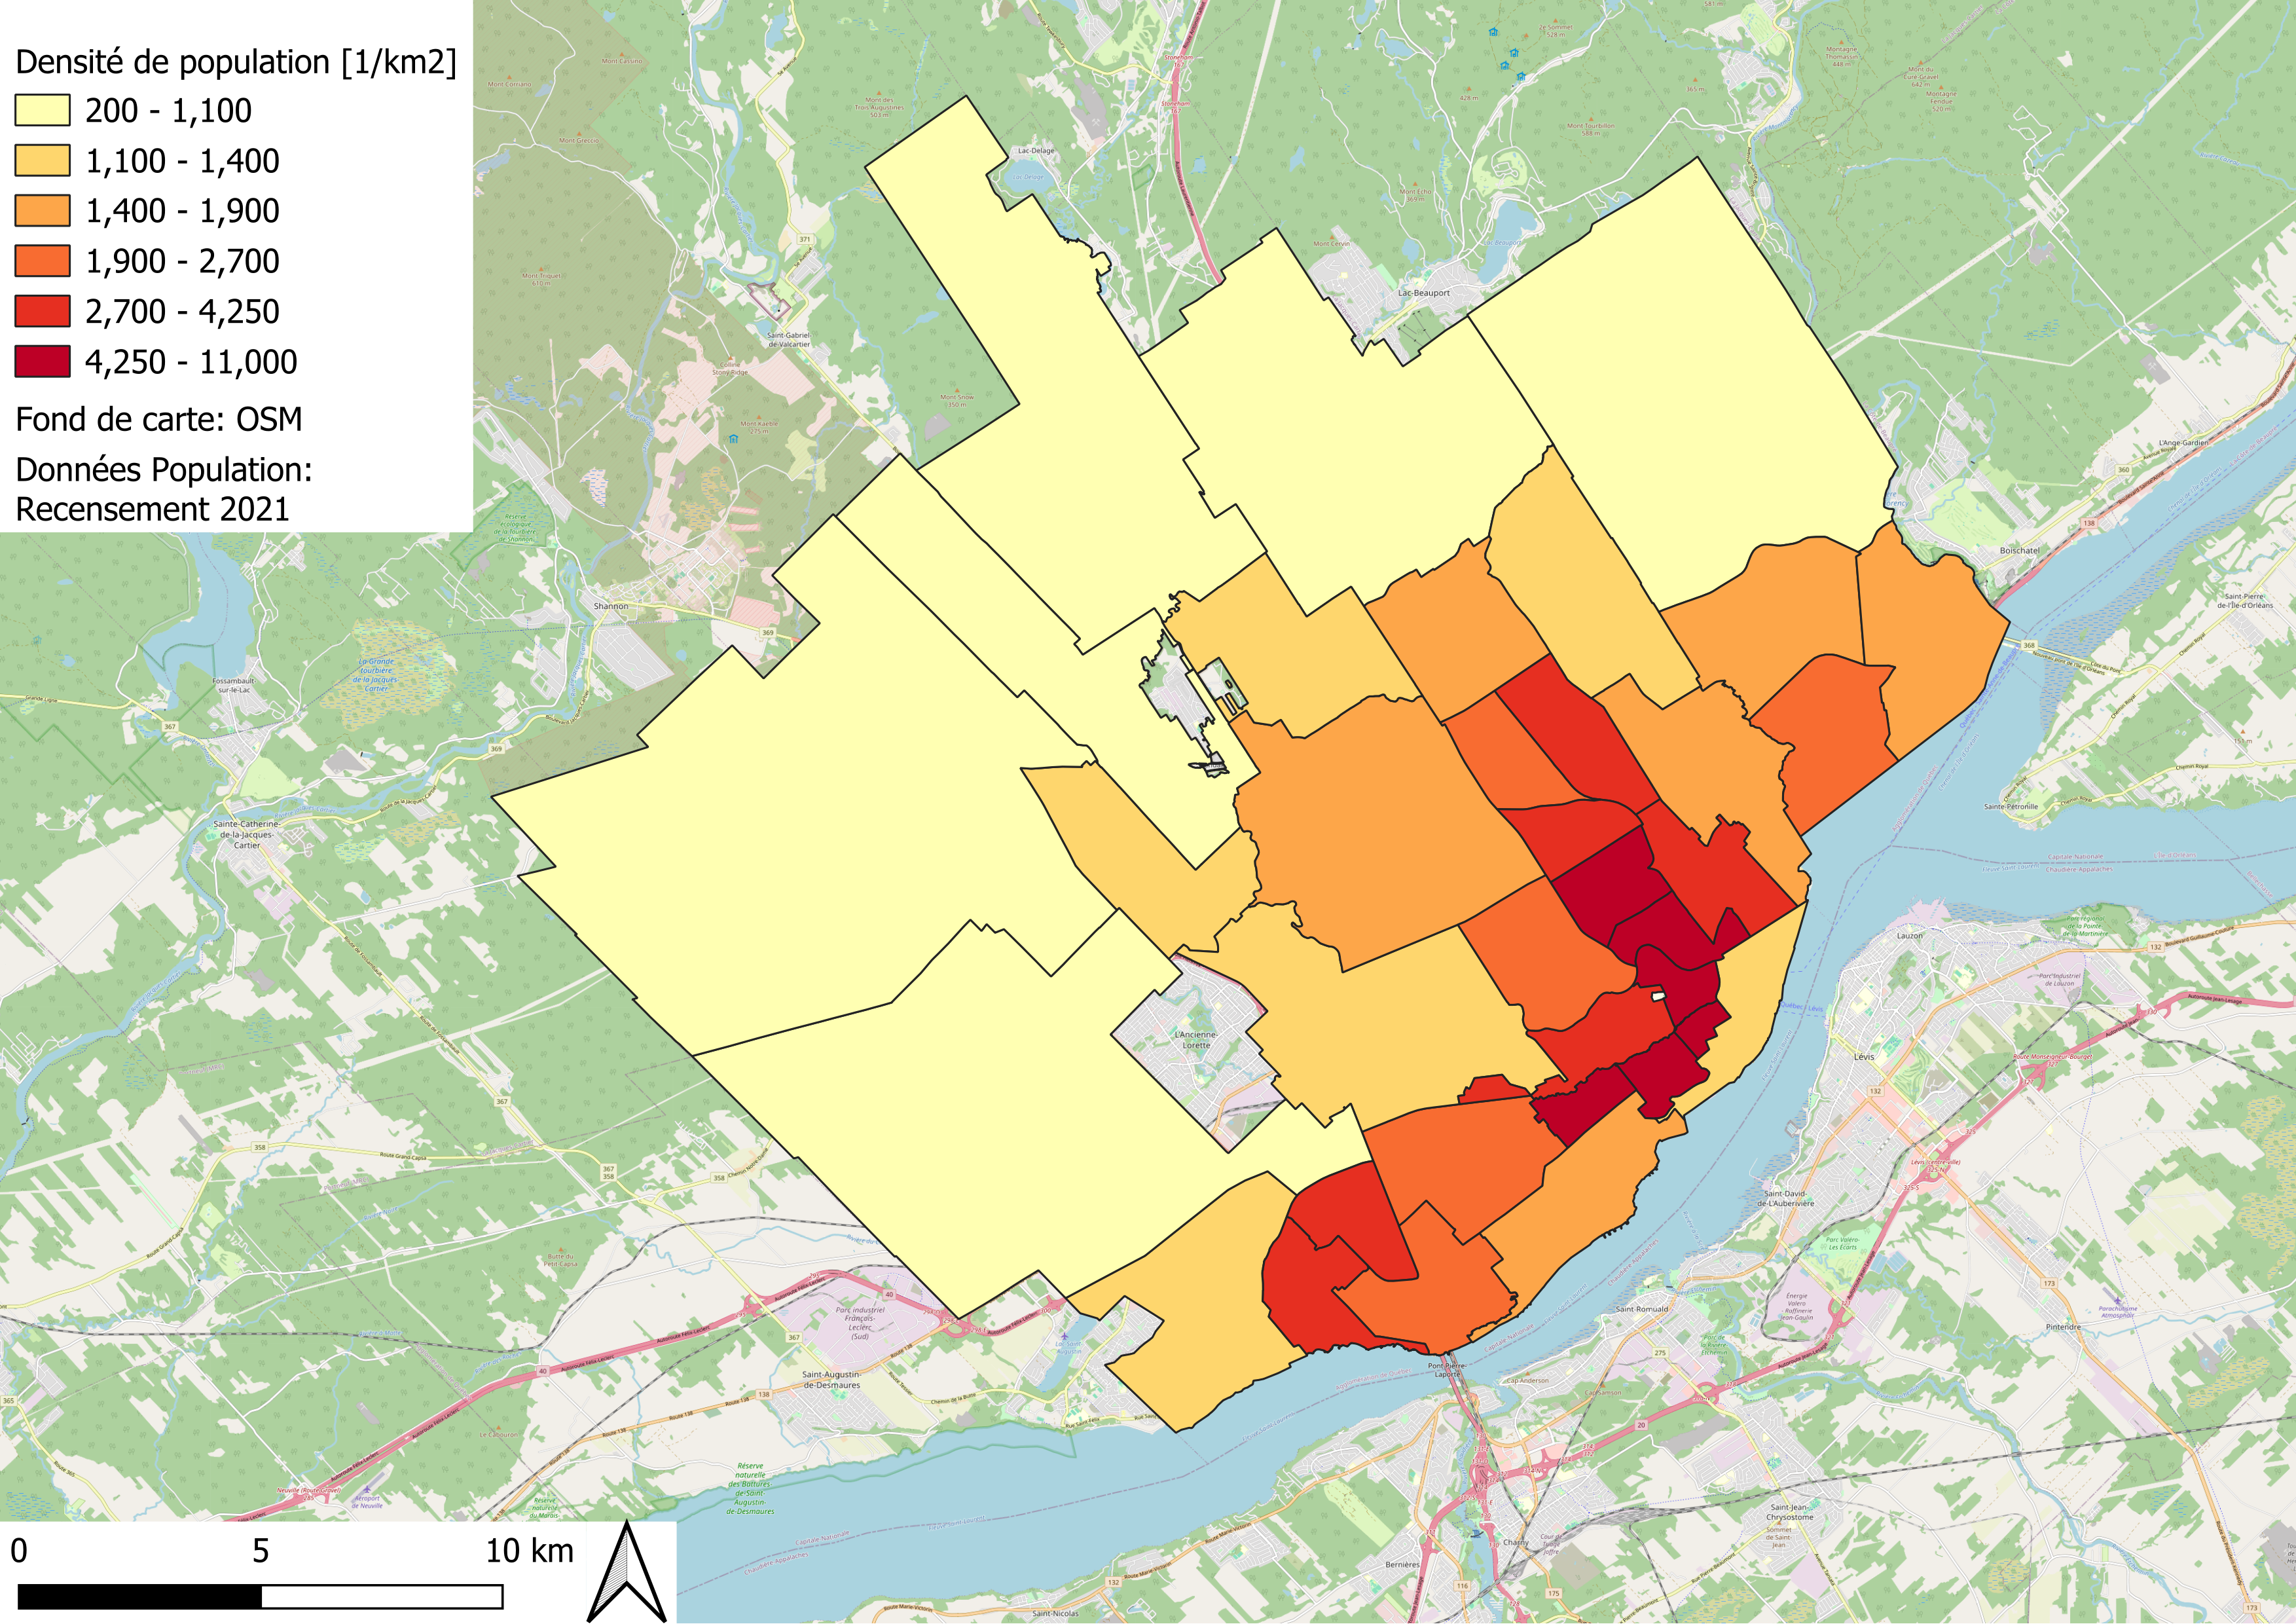
\includegraphics[width=0.9\linewidth]{images/densite-pop.png}
        \caption{Population}
        \label{fig:dens-pop}
    \end{subfigure}
    
    \begin{subfigure}[b]{0.725\textwidth}
        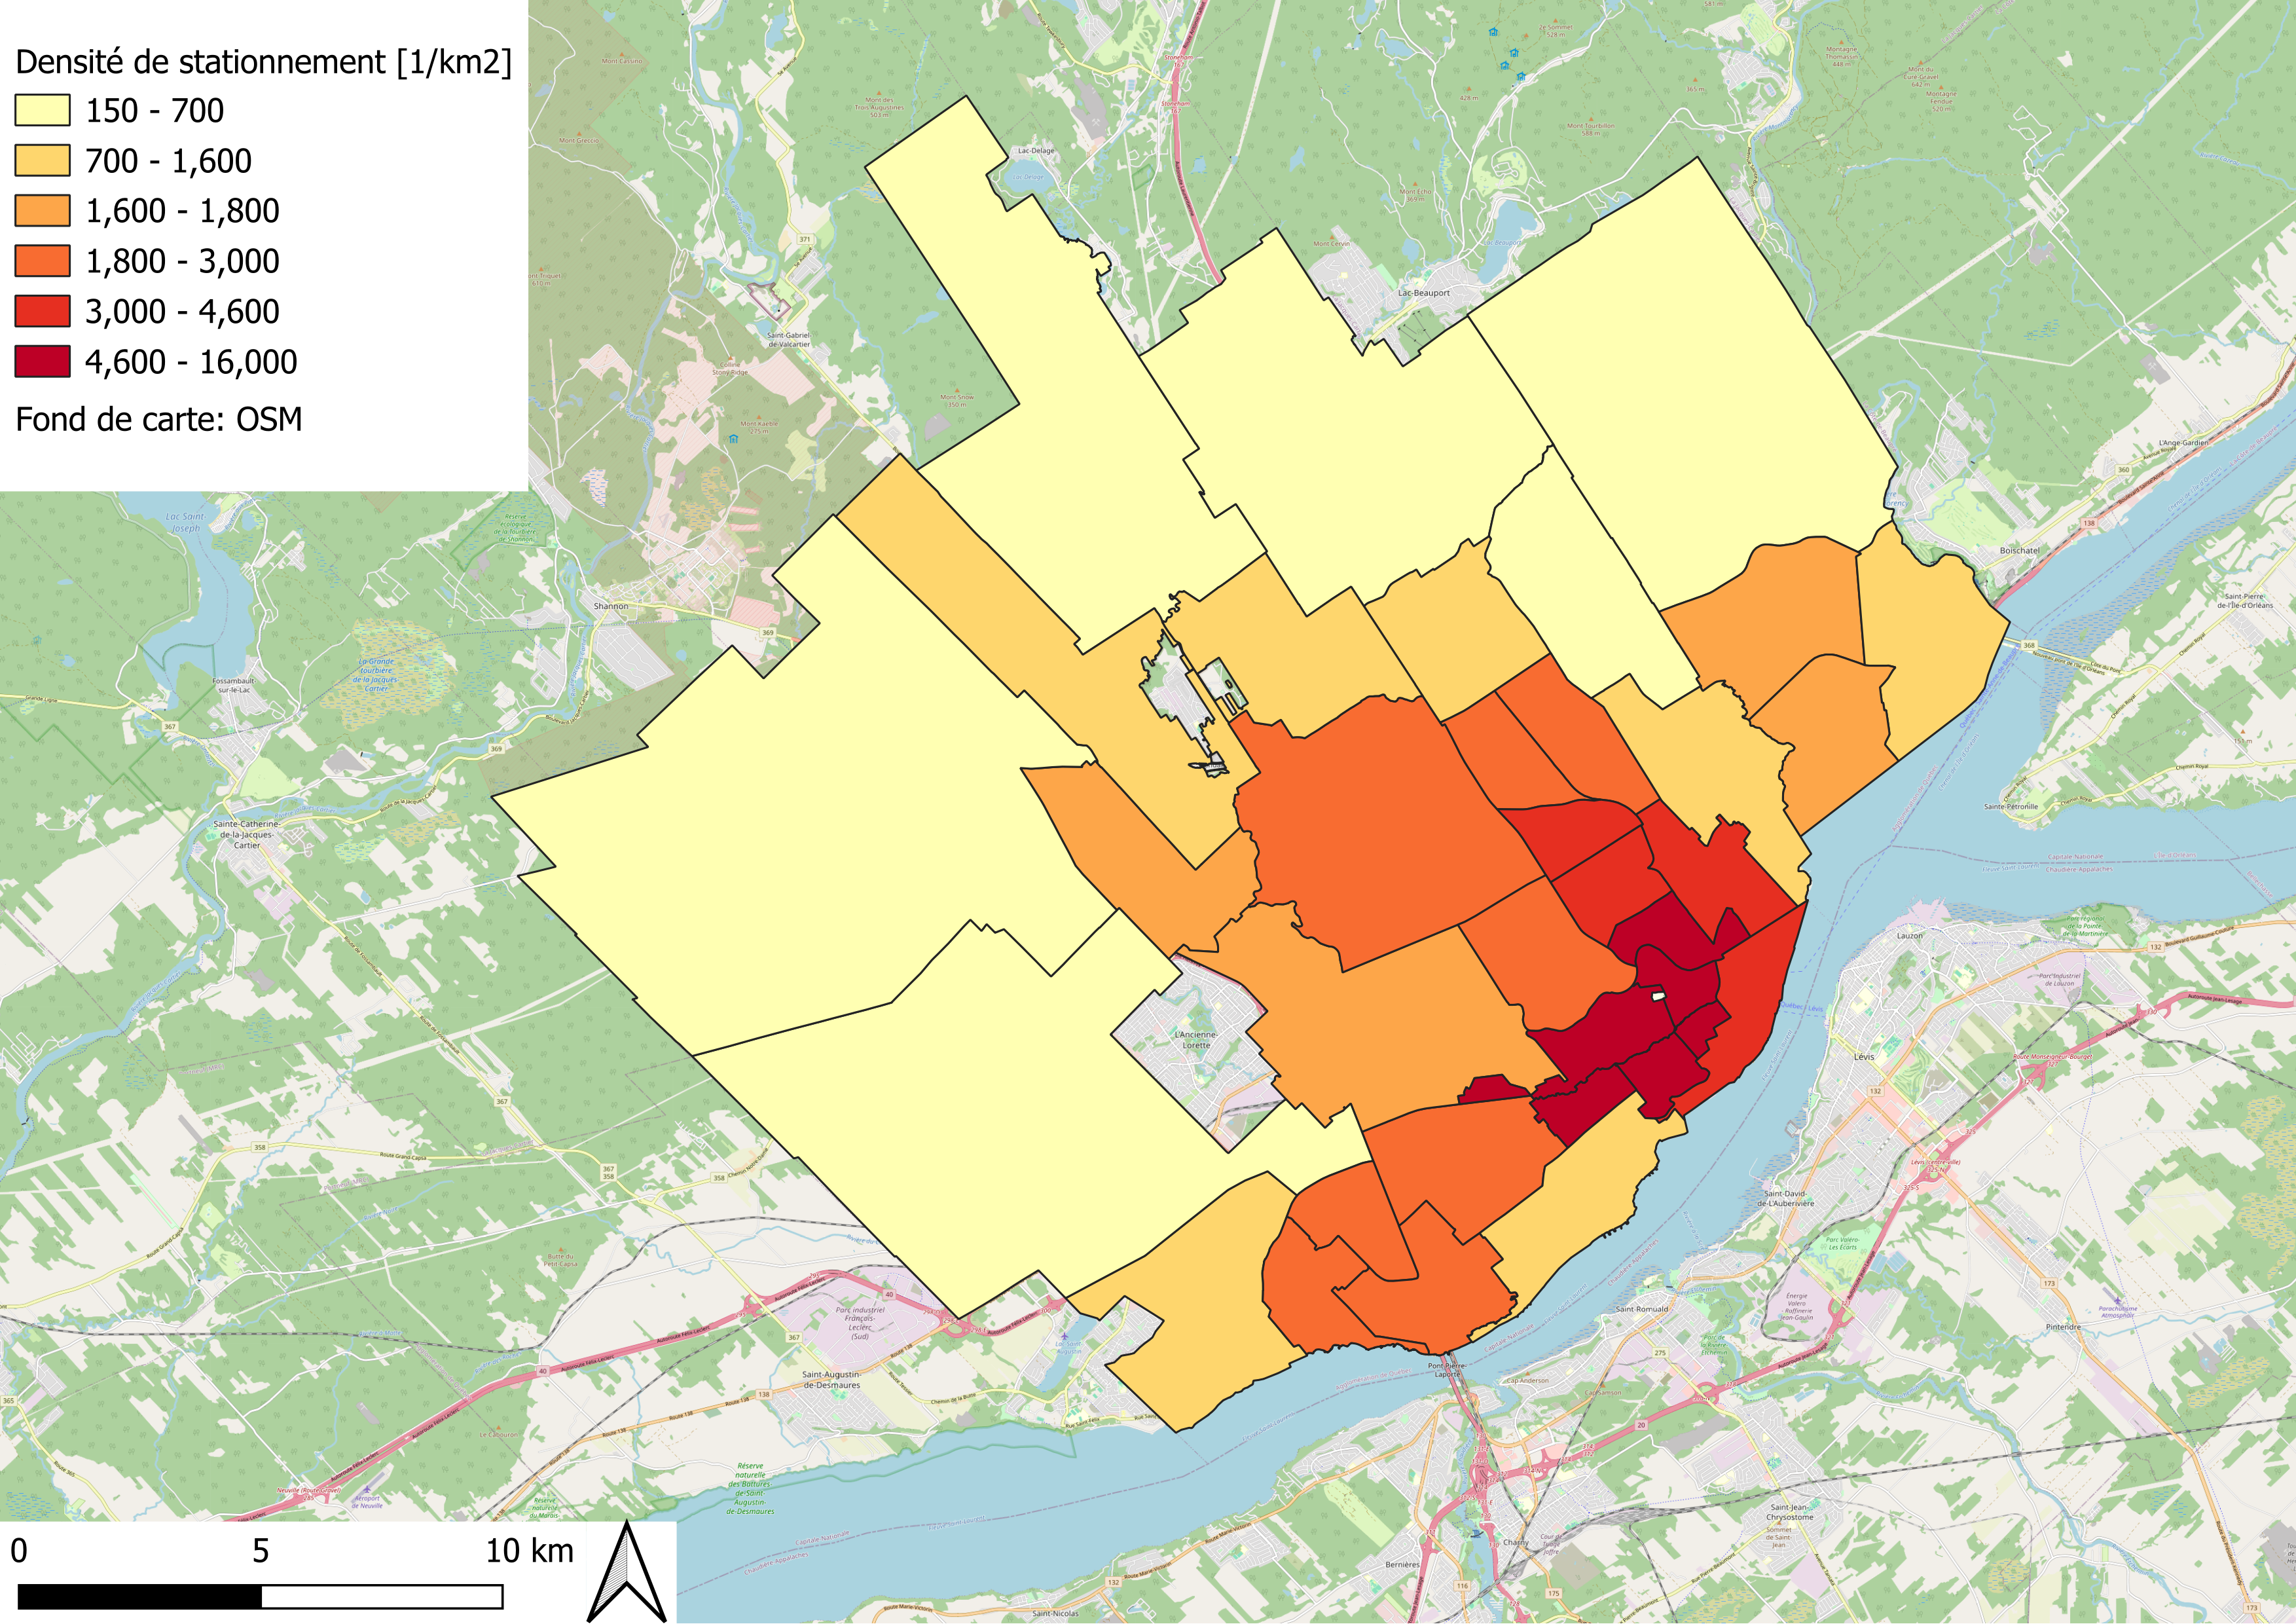
\includegraphics[width=0.9\linewidth]{images/densite-stat-reg.png}
        \caption{Stationnement}
        \label{fig:dens-stat}
    \end{subfigure}
    \caption{Distribution de la densité de stationnement et de population sur le territoire}
\end{figure}\FloatBarrier
La distribution de la capacité de stationnement entre les différentes utilisations du sol n'est pas la même selon les quartiers comme le montre la figure \ref{fig:dist-stat-quart-util}.\par

\begin{figure}[!h]
    \centering
    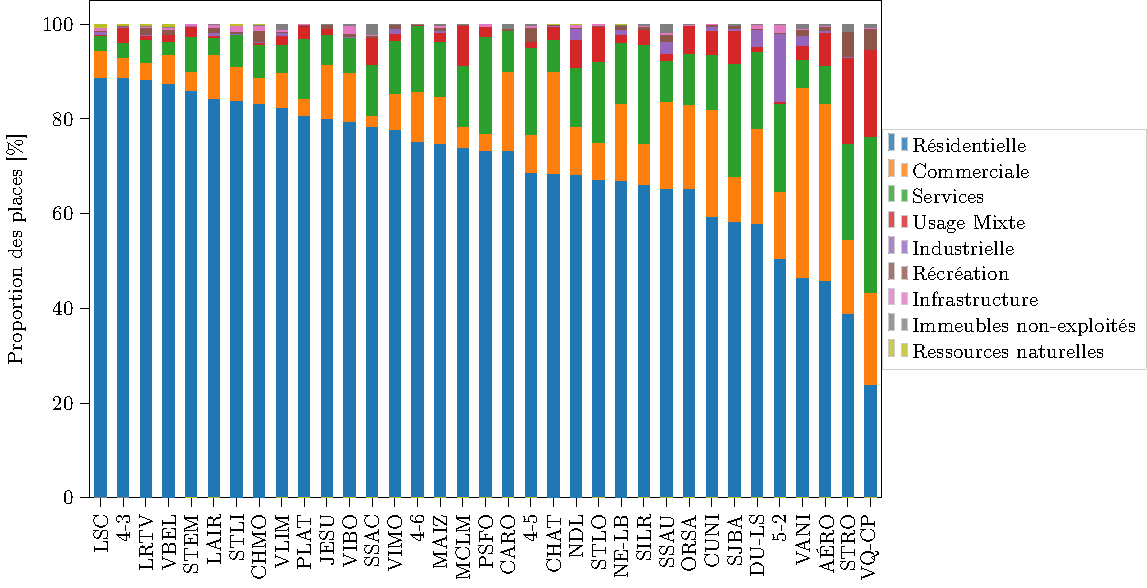
\includegraphics[width=1\linewidth]{figures/distr-inv-prop-quart-util.pdf}
    \caption{Distribution du nombre de places prédites par quartier et usage du sol}
    \label{fig:dist-stat-quart-util}
\end{figure}
Maintenant qu'un bref portrait de la prédiction du parc de stationnement a été dressé. La section suivante fera l'évaluation de la performance du modèle de prédiction.